% Characters of Z/8 on the unit circle. Generated by a short script.
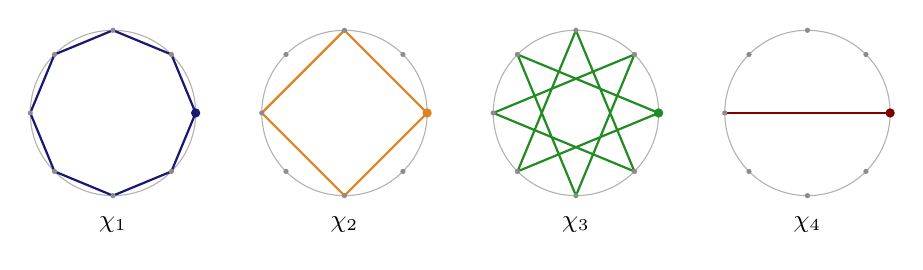
\begin{tikzpicture}[scale=1.05]
\draw[black!30] (0.0,0) circle (1);
\draw[MidnightBlue,thick] (1.0000,0.0000) -- (0.7071,0.7071) -- (0.0000,1.0000) -- (-0.7071,0.7071) -- (-1.0000,0.0000) -- (-0.7071,-0.7071) -- (-0.0000,-1.0000) -- (0.7071,-0.7071) -- (1.0000,-0.0000);
\fill[black!45] (1.0000,0.0000) circle (0.9pt);
\fill[black!45] (0.7071,0.7071) circle (0.9pt);
\fill[black!45] (0.0000,1.0000) circle (0.9pt);
\fill[black!45] (-0.7071,0.7071) circle (0.9pt);
\fill[black!45] (-1.0000,0.0000) circle (0.9pt);
\fill[black!45] (-0.7071,-0.7071) circle (0.9pt);
\fill[black!45] (-0.0000,-1.0000) circle (0.9pt);
\fill[black!45] (0.7071,-0.7071) circle (0.9pt);
\fill[MidnightBlue] (1.0000,0) circle (1.6pt);
\node[font=\small] at (0.0,-1.35) {$\chi_1$};
\draw[black!30] (2.8,0) circle (1);
\draw[BurntOrange!90!black,thick] (3.8000,0.0000) -- (2.8000,1.0000) -- (1.8000,0.0000) -- (2.8000,-1.0000) -- (3.8000,-0.0000) -- (2.8000,1.0000) -- (1.8000,0.0000) -- (2.8000,-1.0000) -- (3.8000,-0.0000);
\fill[black!45] (3.8000,0.0000) circle (0.9pt);
\fill[black!45] (3.5071,0.7071) circle (0.9pt);
\fill[black!45] (2.8000,1.0000) circle (0.9pt);
\fill[black!45] (2.0929,0.7071) circle (0.9pt);
\fill[black!45] (1.8000,0.0000) circle (0.9pt);
\fill[black!45] (2.0929,-0.7071) circle (0.9pt);
\fill[black!45] (2.8000,-1.0000) circle (0.9pt);
\fill[black!45] (3.5071,-0.7071) circle (0.9pt);
\fill[BurntOrange!90!black] (3.8000,0) circle (1.6pt);
\node[font=\small] at (2.8,-1.35) {$\chi_2$};
\draw[black!30] (5.6,0) circle (1);
\draw[ForestGreen,thick] (6.6000,0.0000) -- (4.8929,0.7071) -- (5.6000,-1.0000) -- (6.3071,0.7071) -- (4.6000,0.0000) -- (6.3071,-0.7071) -- (5.6000,1.0000) -- (4.8929,-0.7071) -- (6.6000,-0.0000);
\fill[black!45] (6.6000,0.0000) circle (0.9pt);
\fill[black!45] (6.3071,0.7071) circle (0.9pt);
\fill[black!45] (5.6000,1.0000) circle (0.9pt);
\fill[black!45] (4.8929,0.7071) circle (0.9pt);
\fill[black!45] (4.6000,0.0000) circle (0.9pt);
\fill[black!45] (4.8929,-0.7071) circle (0.9pt);
\fill[black!45] (5.6000,-1.0000) circle (0.9pt);
\fill[black!45] (6.3071,-0.7071) circle (0.9pt);
\fill[ForestGreen] (6.6000,0) circle (1.6pt);
\node[font=\small] at (5.6,-1.35) {$\chi_3$};
\draw[black!30] (8.399999999999999,0) circle (1);
\draw[Maroon,thick] (9.4000,0.0000) -- (7.4000,0.0000) -- (9.4000,-0.0000) -- (7.4000,0.0000) -- (9.4000,-0.0000) -- (7.4000,0.0000) -- (9.4000,-0.0000) -- (7.4000,0.0000) -- (9.4000,-0.0000);
\fill[black!45] (9.4000,0.0000) circle (0.9pt);
\fill[black!45] (9.1071,0.7071) circle (0.9pt);
\fill[black!45] (8.4000,1.0000) circle (0.9pt);
\fill[black!45] (7.6929,0.7071) circle (0.9pt);
\fill[black!45] (7.4000,0.0000) circle (0.9pt);
\fill[black!45] (7.6929,-0.7071) circle (0.9pt);
\fill[black!45] (8.4000,-1.0000) circle (0.9pt);
\fill[black!45] (9.1071,-0.7071) circle (0.9pt);
\fill[Maroon] (9.4000,0) circle (1.6pt);
\node[font=\small] at (8.399999999999999,-1.35) {$\chi_4$};
\end{tikzpicture}
